\newpage
\usecasegenerico{Effettua registrazione}
\label{usecase:Effettua registrazione}

\begin{figure}[h]
	\centering
	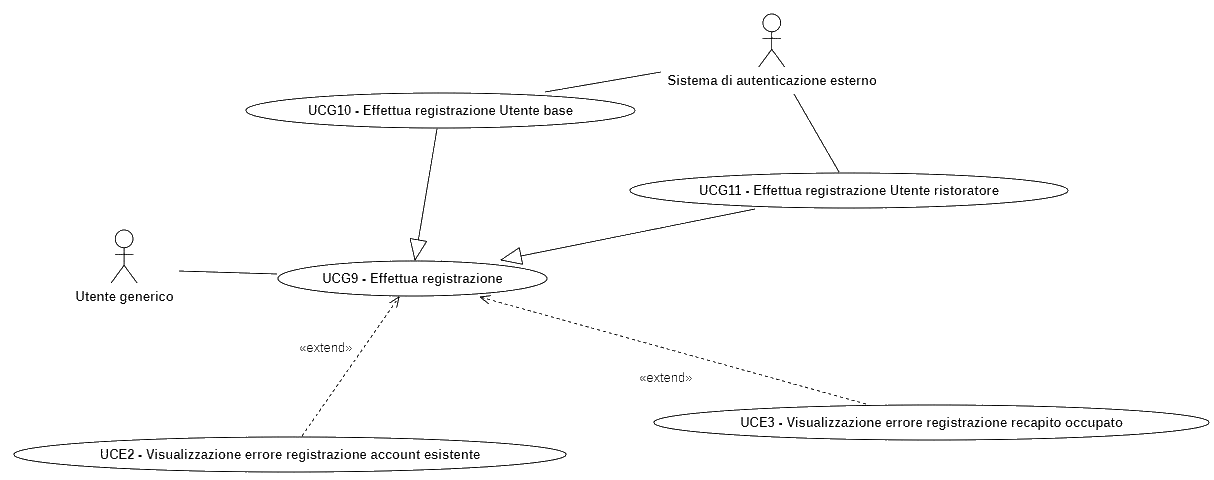
\includegraphics[width=0.999\textwidth]{./uml/UCG9-10-11.png} 
	\caption{Effettua registrazione}
	\label{fig:UCG9-10-11}
  \end{figure}

\begin{itemize}
	\item \textbf{Descrizione:} Un Utente generico decide di registrarsi all'interno della \textit{web app}. 
    Durante questa procedura, l'utente è tenuto a selezionare la tipologia di \textit{account} desiderata tra le due opzioni disponibili: Utente base o Utente ristoratore.
    Può raggiungere la pagina di registrazione di uno dei due tipi di utenza tramite l'impiego di \textit{link} che lo reindirizzano alla pagina di registrazione di sua scelta. 
    Successivamente, all'utente viene richiesto di inserire una serie di dati correlati alla registrazione e specifici alla tipologia di utenza scelta.

	\item \textbf{Attore principale:} Utente generico.
	\item \textbf{Attore secondario:} Sistema di autenticazione esterno.
	\item \textbf{Precondizioni:}
        \begin{itemize}
            \item L'Utente generico è connesso al Sistema.
            \item L'Utente generico non dispone di un \textit{account}.
        \end{itemize}
	\item \textbf{Postcondizioni:}
        \begin{itemize} 
            \item L'Utente generico ha creato con successo un \textit{account} scegliendo tra le opzioni disponibili:
            \begin{itemize}
                \item Utente ristoratore.
                \item Utente base.
            \end{itemize}
            \item Tutte le informazioni relative al nuovo \textit{account} sono memorizzate all'interno del Sistema.
            \item L'Utente autenticato viene reindirizzato alla pagina \textit{Home} di pertinenza.
        \end{itemize}


	\item \textbf{Scenario principale:}
	      \begin{enumerate}
		      \item L'Utente generico seleziona la tipologia di \textit{account} da creare: 
		      \begin{itemize}
				\item Utente base (vedi \autoref{usecase:Effettua registrazione Utente base}).
				\item Utente ristoratore (vedi \autoref{usecase:Effettua registrazione Utente ristoratore}).
			  \end{itemize} 
              \item Il Sistema memorizza con successo il nuovo \textit{account} creato;
		      \item L'utente è autenticato e viene reindirizzato alla pagina \textit{Home} corrispondente.
	      \end{enumerate}
		
    \item \textbf{Scenario secondario:}
                \begin{enumerate}
                    \item La registrazione fallisce per due ragioni:
                    \begin{itemize}
                        \item La registrazione fallisce a causa dell'esistenza di un \textit{account} preesistente con le stesse credenziali inserite (vedi \autoref{usecase:Errore registrazione account esistente}).
                        \item La registrazione non va a buon fine in quanto l'Utente Ristoratore ha inserito un recapito del ristorante già occupato (vedi \autoref{usecase:Errore registrazione recapito occupato}).
                    \end{itemize}
                    \item L'Utente generico viene nuovamente indirizzato alla pagina di accesso.
                \end{enumerate}	
          
\end{itemize}